\section{Other experiments}
After obtaining a better understanding of how \acp{GAN} work from the previous experiments, the next goal was to try and apply them to the Flowers and CelebA datasets in order to see if the knowledge could be transferred to these situations and if it would be possible to produce good results.

However, the images in these datasets were of too high resolutions for processing using the available machine, knowing this, they both were reduced to the more manageable resolutions of $48\times48$. The Flowers dataset was created in such a way that the shorter dimension has always 500 pixels, using this fact, the longer dimensions were center cropped to be of the same size and the resulting images were scaled down to the desired lower resolution. \autoref{fig:flowers_reduced} shows some samples in this reduced dataset.
\begin{figure}[hbt]
    \centering
    \caption{Reduced Flowers dataset}
    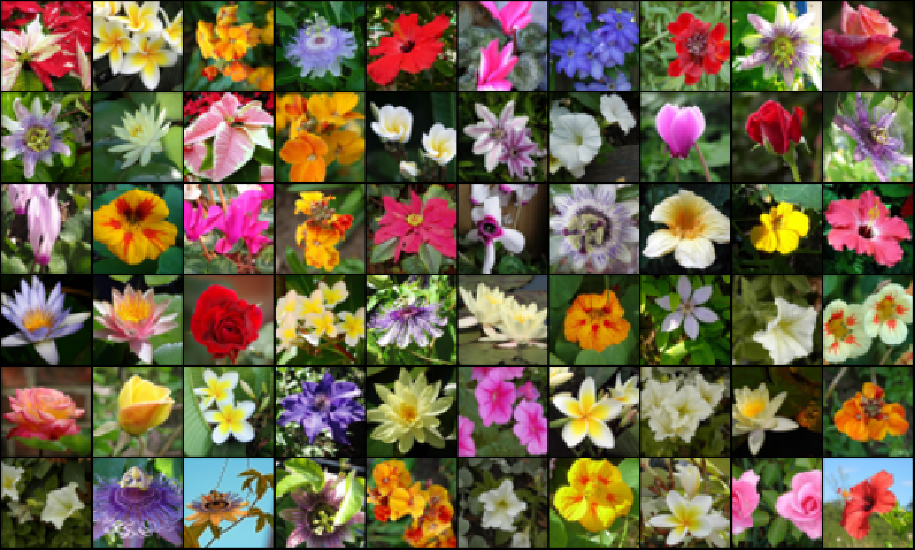
\includegraphics[width=0.7\textwidth]{chapters/Experiments/Other/Flowers_reduced.pdf}
    \fonte{From the author (2021)}
    \label{fig:flowers_reduced}
\end{figure}

The CelebA dataset has all images of height $218$ and width $178$, besides this, all images have the faces centered in the approximately same spot. Using this fact, the central part of the face was cropped, the horizontal pixels ranged from 41 to 137 and the vertical ones ranged from 85 to 181 (count starts from 0). Theses values were selected to best match the face position and the cropping resulted in $96\times96$ images, which were then downscaled to the desired resolution. \autoref{fig:celeba_reduced} shows samples from this reduced dataset.
\begin{figure}[hbt]
    \centering
    \caption{Reduced CelebA dataset}
    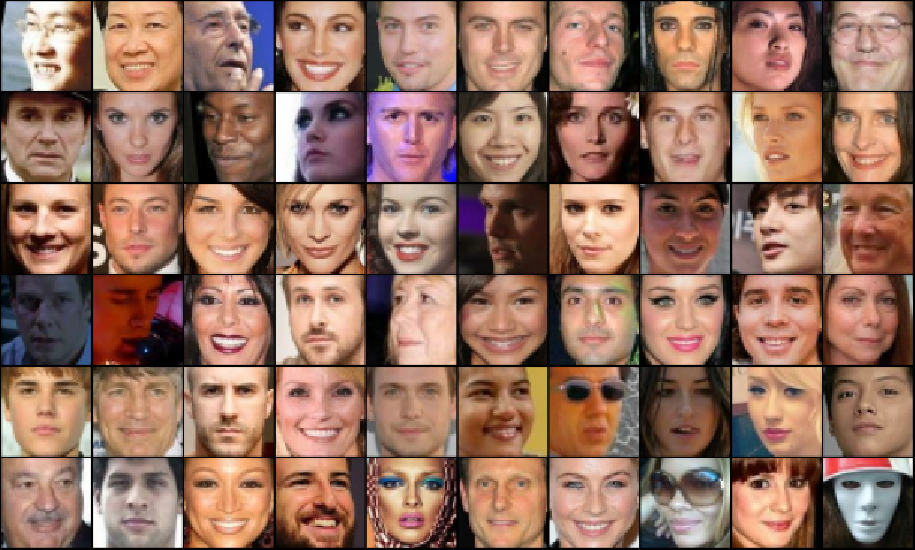
\includegraphics[width=0.7\textwidth]{chapters/Experiments/Other/CelebA_reduced.pdf}
    \fonte{From the author (2021)}
    \label{fig:celeba_reduced}
\end{figure}

These reduced datasets were use to test another three models, however, the \gls{CS} and \gls{FCD} metrics were not calculated for these experiments. Calculating the metrics would often cause memory problems even when evaluating models trained on \gls{CIFAR}-10, evaluating the CelebA models would be impossible given the size of the dataset. 

There was an attempt to use the Inception v3 model to calculate the \gls{IS} and \gls{FID} for the CelebA models, although it was possible to find a solution that would not cause memory issues, it was significantly slower and the results were completely senseless. Maybe a deeper familiarity with Tensorflow would produce a viable solution, but for this case the metrics were ignored and the results are only to be evaluated qualitatively.

\subsection{Flowers with DCGAN}
Since the Flowers dataset contained only a small number of images, it was relatively quick to test different configurations and see if the results were promising. It was found that batch normalization did not produce good results, and that only nearest neighbour upsampling was a valid upscaling technique.

This experiment showed the most extreme cases of checkerboard artifacts that can occur when using transposed convolutions, no set of hyperparameters that could avoid this was found, even following the recommendations given by \textcite{deconvolutionArtifacts2016} did not proved fruitful. \autoref{fig:flowers_trpconv} shows what the generator has produced after 20 epochs of training, it is even possible to see a hint of flowers behind the grid artifact. 
\begin{figure}[hbt]
    \centering
    \caption{DCGAN with transposed convolutions trained on Flowers}
    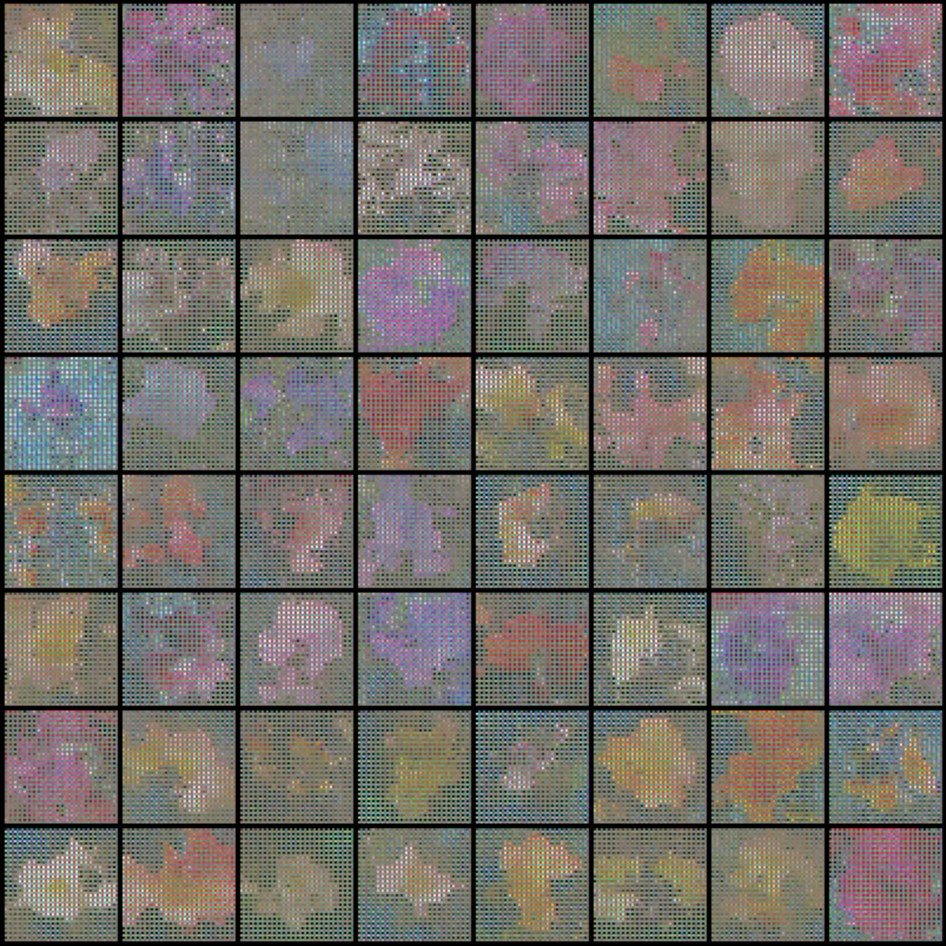
\includegraphics[width=0.5\textwidth]{chapters/Experiments/Other/flowers_trpconv.png}
    \fonte{From the author (2021)}
    \label{fig:flowers_trpconv}
\end{figure}

Bilinear upsampling would create another pattern, the images generated would be oddly smooth everywhere. The generator was able to create some basic representation, by looking at a distance it is even possible to see a hint of the images being generated, but looking closely only very circular shapes are seen. \autoref{fig:flowers_bilinear} shows samples from the bilinear upsampling generator after 20 epochs of training.
\begin{figure}[hbt]
    \centering
    \caption{DCGAN with bilinear upsampling trained on Flowers}
    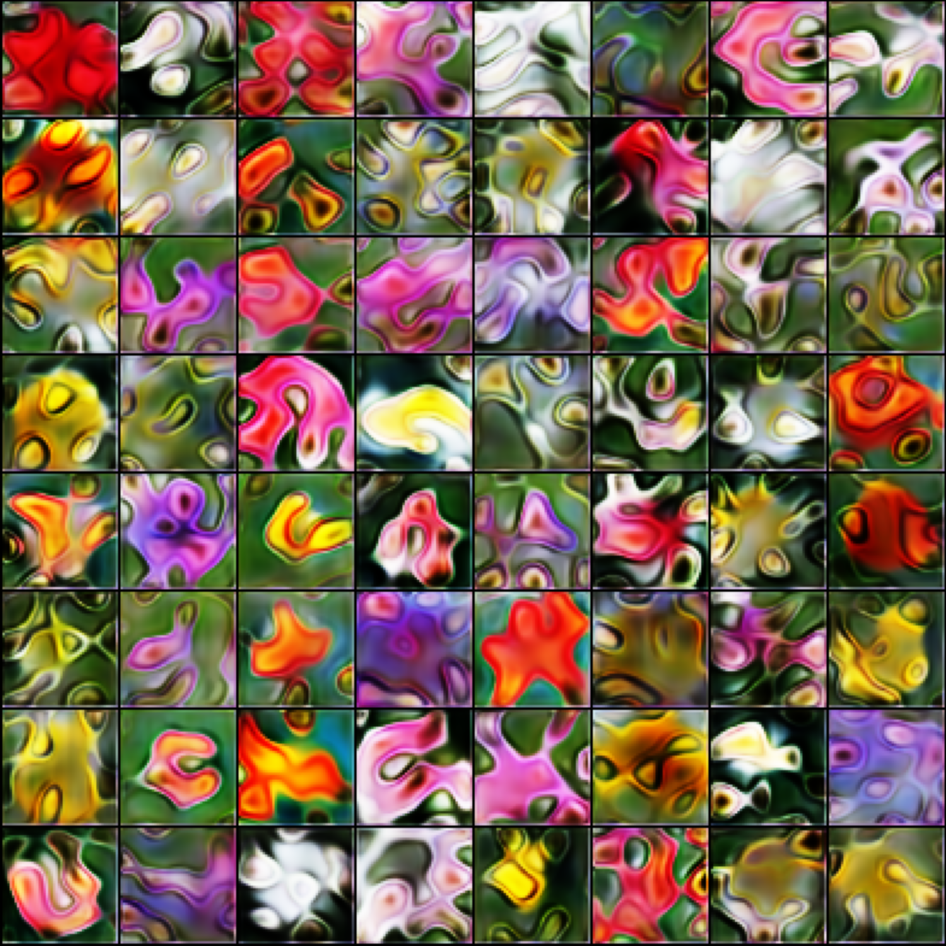
\includegraphics[width=0.45\textwidth]{chapters/Experiments/Other/flowers_bilinear.png}
    \fonte{From the author (2021)}
    \label{fig:flowers_bilinear}
\end{figure}

This was not mentioned until yet, but this behaviour of the bilinear upsampling was universally seen in all tests made on \gls{CIFAR}-10, although to a lesser extent. This is the author's hypothesis as to why the \gls{MNIST} tests showed good results for this type of upsampling, since the digits already have some smoothness to their design, this technique fits particularly well to this case. Transposed convolutions and nearest neighbour upsampling usually produce more rough and realistic looking images, explaining the fact of why they performed better on the other datasets.

Lastly, the nearest neighbour upsampling is the only one who does not produce checkerboard artifacts while still upscaling the images to a more realistic look, this configuration showed the best results and was trained the longest until 100 epochs. The flowers generated by this model after the end of training are shown in \autoref{fig:flowers_nearest}.
\begin{figure}[hbt]
    \centering
    \caption{DCGAN with nearest neighbour upsampling trained on Flowers}
    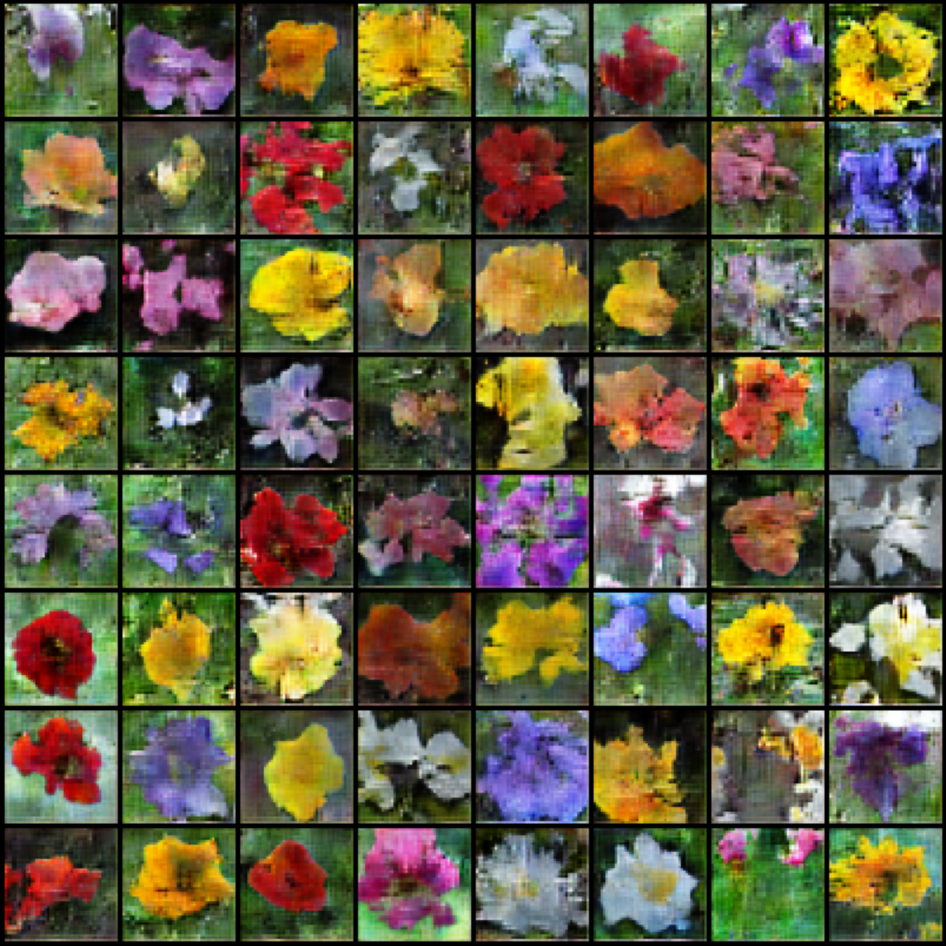
\includegraphics[width=0.45\textwidth]{chapters/Experiments/Other/flowers_nearest.png}
    \fonte{From the author (2021)}
    \label{fig:flowers_nearest}
\end{figure}

\subsection{Faces with DCGAN}
This model was considerably slower to train, so most of the decisions over its design were made before training, based on the previous results. Of particular importance, the generator used nearest neighbour upsampling and batch normalization, the latent space had $256$ dimensions, and the labels were smoothed to the value $0.9$. Due to the time needed for training, this model was not trained to near convergence, but only for 20 epochs.

Since the results tend to fluctuate, it is common to see previous epochs producing better results, for this reason \autoref{fig:dcgan_celeba} shows samples from the last three epochs of training. Given their small size, there are some particularly realistic looking images produced by the generator in this set, but it still produces many deformed figures and incomplete eyeglasses. 
\begin{figure}[hbt]
    \caption{DCGAN trained on CelebA}
    \centering
        \begin{subfigure}[b]{0.3\textwidth}
        \centering
        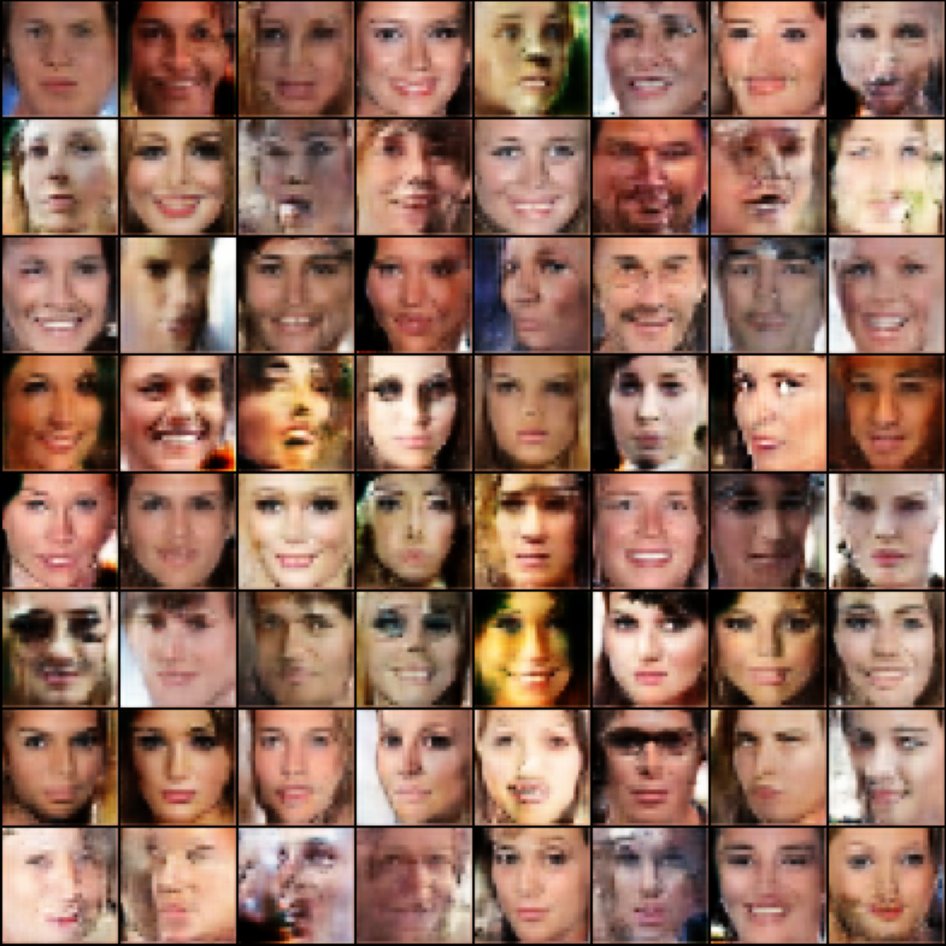
\includegraphics[width=\textwidth]{chapters/Experiments/Other/dcgan_celeba18.png}
        \caption{Epoch 18}
        \end{subfigure}
    \hfill
        \begin{subfigure}[b]{0.3\textwidth}
        \centering
        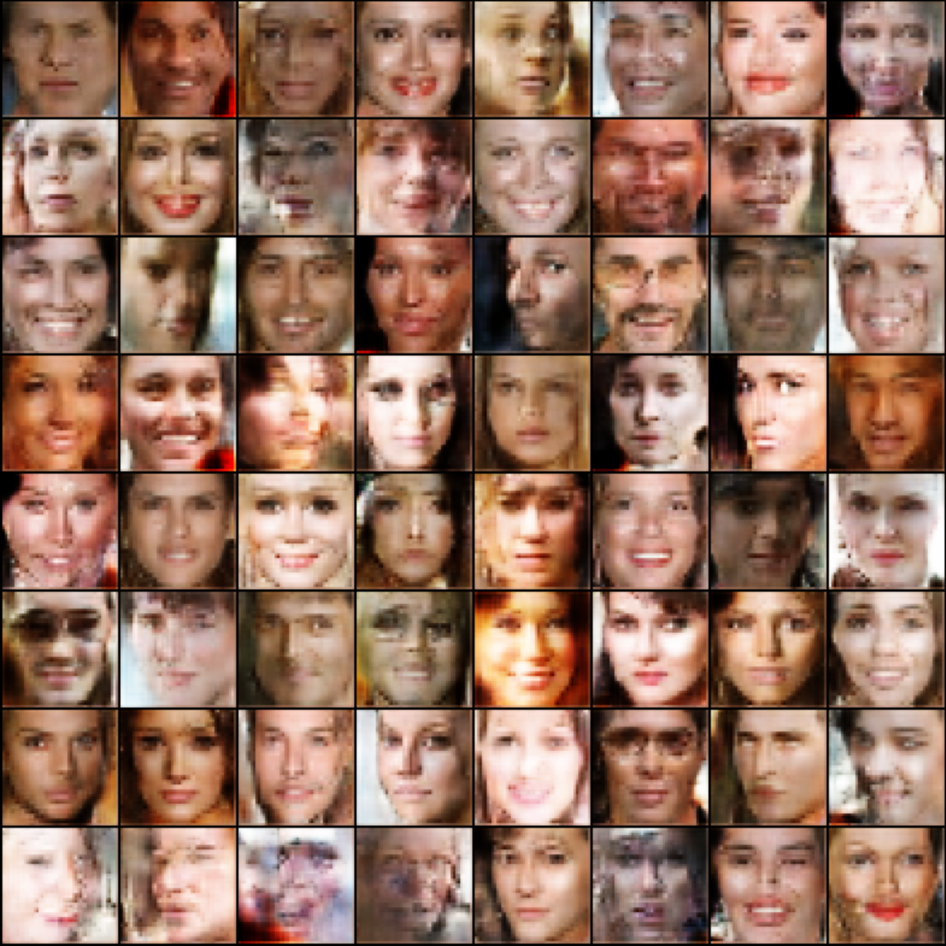
\includegraphics[width=\textwidth]{chapters/Experiments/Other/dcgan_celeba19.png}
        \caption{Epoch 19}
        \end{subfigure}
    \hfill
        \begin{subfigure}[b]{0.3\textwidth}
        \centering
        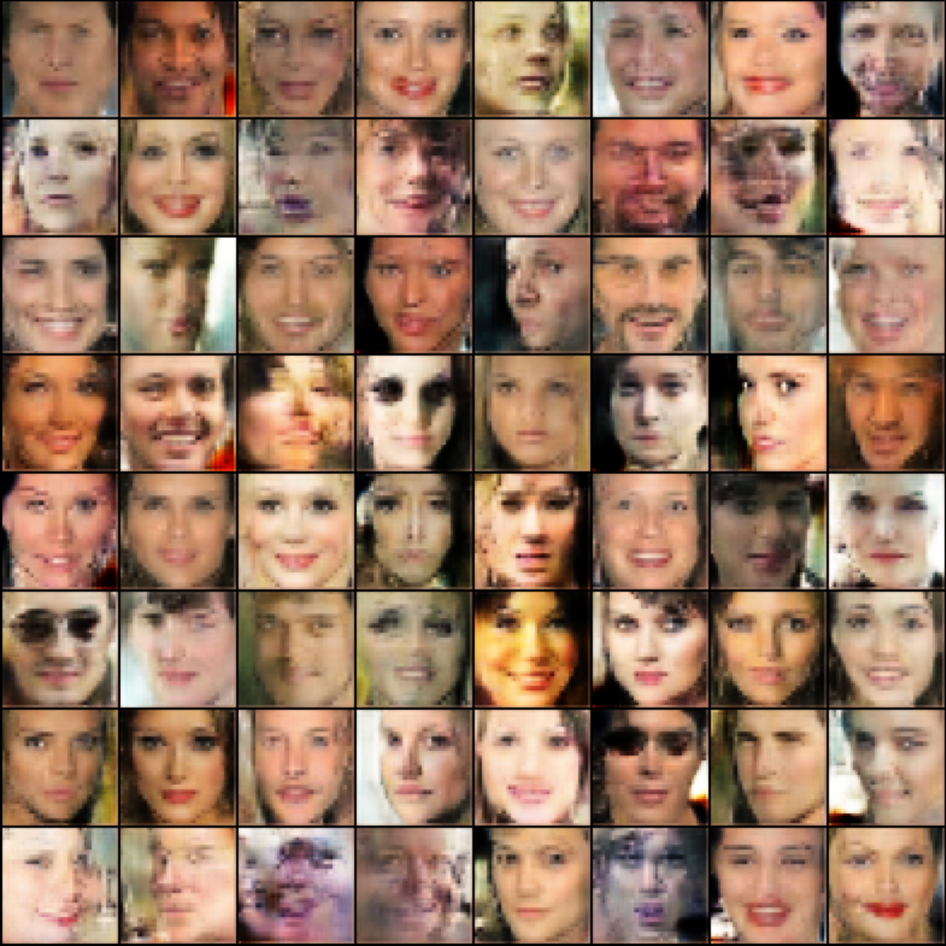
\includegraphics[width=\textwidth]{chapters/Experiments/Other/dcgan_celeba20.png}
        \caption{Epoch 20}
        \end{subfigure}
    \fonte{From the author (2021)}
    \label{fig:dcgan_celeba}
\end{figure}



\subsection{Faces with WGAN-GP}
The authors of \gls{WGAN-GP} mention that ``For equivalent architectures, our method achieves comparable sample quality to the standard GAN objective'' \cite{wgan-gp2017} and follow by mentioning the increased stability of the model as an advantage. The previous experiments have supported both of these claims, since the models have shown similar results with the DCGAN for all datasets tested and the hyperparameter choices showed consistent quality in different situations. Given this knowledge, the goal for this experiment was to see if the \gls{WGAN-GP} could scale better than the \gls{DCGAN} for this face generation problem.

\begin{figure}[hbt]
    \caption{WGAN-GP trained on CelebA}
    \centering
        \begin{subfigure}[b]{0.3\textwidth}
        \centering
        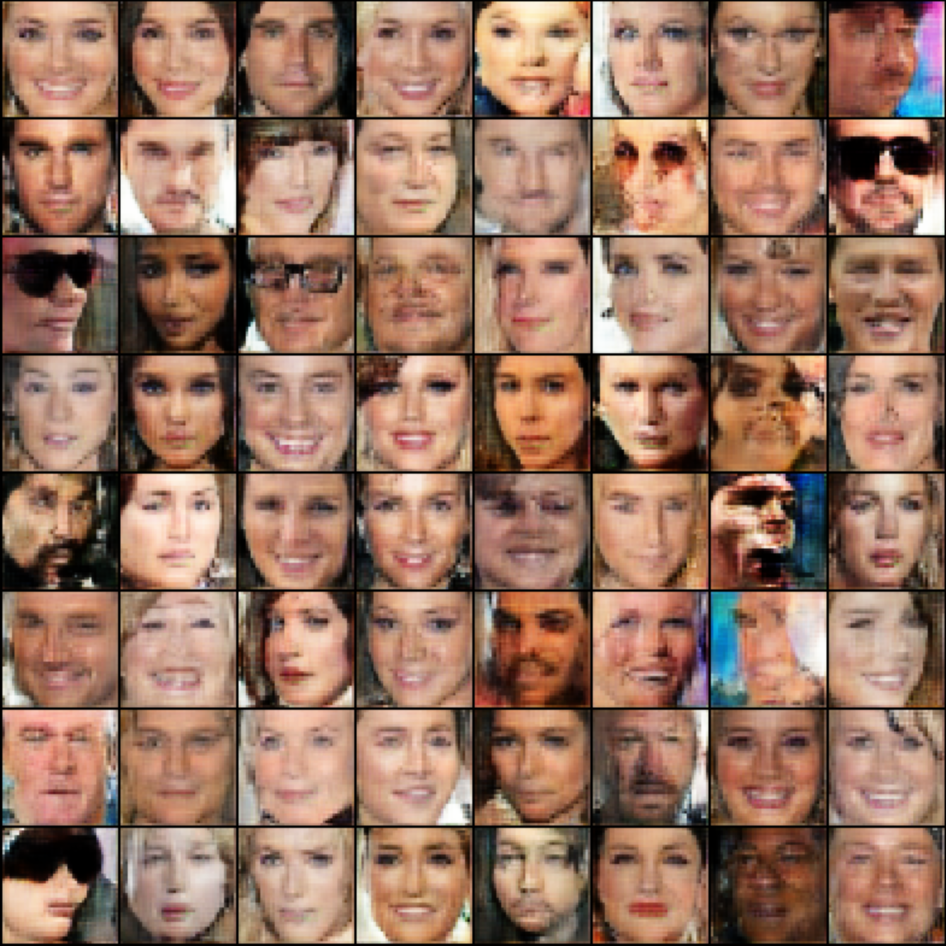
\includegraphics[width=\textwidth]{chapters/Experiments/Other/wgan_gp_celeba18.png}
        \caption{Epoch 18}
        \end{subfigure}
    \hfill
        \begin{subfigure}[b]{0.3\textwidth}
        \centering
        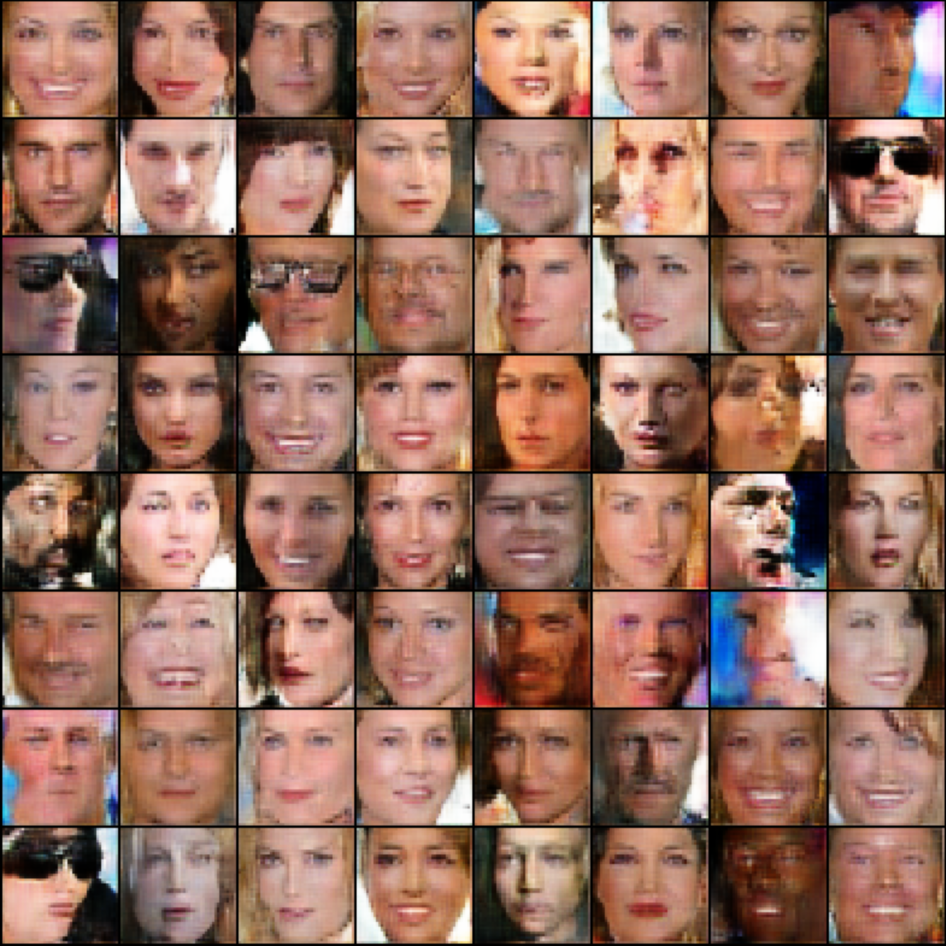
\includegraphics[width=\textwidth]{chapters/Experiments/Other/wgan_gp_celeba19.png}
        \caption{Epoch 19}
        \end{subfigure}
    \hfill
        \begin{subfigure}[b]{0.3\textwidth}
        \centering
        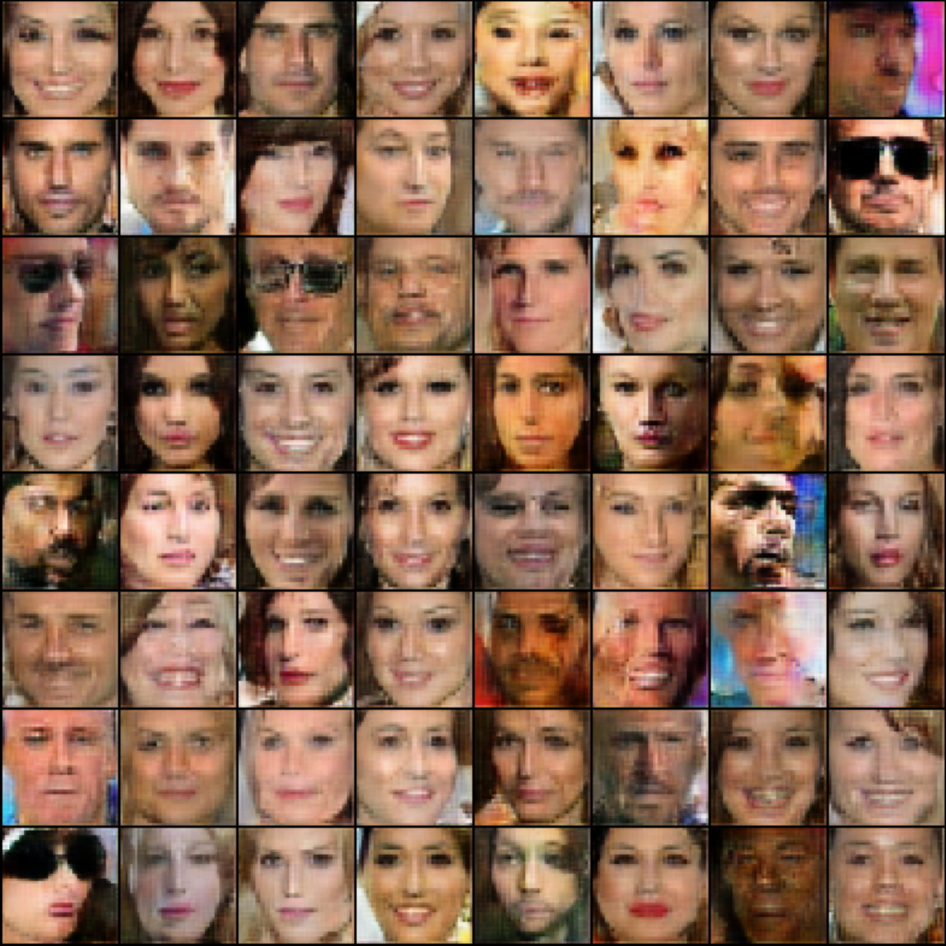
\includegraphics[width=\textwidth]{chapters/Experiments/Other/wgan_gp_celeba20.png}
        \caption{Epoch 20}
        \end{subfigure}
    \fonte{From the author (2021)}
    \label{fig:wgan_gp_celeba}
\end{figure}

This model is very much alike the previous one, only the discriminator was changed for a similar critic and the loss was changed as required by the \gls{WGAN-GP} architecture. The batch normalization was also removed from the generator since it was found to produce some artifacts that reduced the image quality. The results from this experiment are shown in \autoref{fig:wgan_gp_celeba}.

By a qualitative analysis it is the opinion of the author that the results from the \gls{WGAN-GP} are generally better, the images seem more realistic and there is less deformations overall.


% \subsection{Latent Space Interpolation}
